%!TEX root = ../thesis.tex

\chapter{Огляд сучасних методів сегментації супутникових знімків}
\label{chap:sem_segm}

У першому розділі даної роботи ми розглянемо постановку
задачі семантичної сегментації, нейромережеві методи, які
застосовують для її розв'язку, а також специфічні проблеми,
які виникають при застосуванні цих методів до супутникових
знімків. Також мова піде про функції помилки та метрики якості
сегментації, які будуть використані у наступних розділах.

\section{Задача семантичної сегментації супутникових знімків}

Серед широко спектру задач, які пов'язані з використанням
супутникових знімків, особливе місце займає задача семантичної
сегментації. Розв'язок даної задачі дозволяє вирішувати такі прикладні задачі,
як, наприклад, детектування вирубки лісів \cite{sat_logging}, класифікацію
сільськогосподарських полів \cite{kussul2017deep}
і відіграє визначну роль у задачах моніторингу навколишнього
середовища та сільського господарства.

\subsection{Постановка задачі сегментації}

Як і інші задачі навчання з учителем, задача семантичної сегментації
передбачає існування навчальної вибірки, тобто набору $X$,
який складається з зображень
$I \in \left( R^C \right)^{H \times W} = \mathcal{I}$ та міток класів
$k \in K$ для кожного пікселя кожного зображення, де $R \subset \R$ --
множина можливих значень кожного каналу пікселя,
$H, W, C$ -- висота, ширина та кількість каналів зображення,
$K = \overline{1, M}$ -- множина класів ($M \in \N$ -- кількість класів).
Зазвичай множина $R = \overline{0, \dots, 255}$, або $R = [0, 1]$.

\begin{definition} \label{def:sem_segm_task}
    Нехай ми маємо навчальну вибірку $X=(I_i, Y_i)_{i=1}^{N}$,
    де $I_i \in \mathcal{I}$, $Y_i \in K^{H \times W}$.
    Задача семантичної сегментації полягає у тому, щоб
    знайти таке відображення
    $f: \mathcal{I} \rightarrow K^{H \times W}$, що деякий функціонал помилки
    $L(f, X)$ приймає мінімальне значення.
\end{definition}

Тобто задача семантичної сегментації є задачею класифікації, але
не цілого зображення, а кожного окремого пікселя.

% \begin{figure}[ht]
%     \centering
%     \begin{subfigure}[b]{0.45\textwidth}
%         \centering
%         \includegraphics[scale=0.5]{../assets/satellite.png}
%         \caption{Вхідне зображення}
%     \end{subfigure}%
%     \begin{subfigure}[b]{0.45\textwidth}
%         \centering
%         \includegraphics[scale=0.5]{../assets/mask.png}
%         \caption{Результат сегментації}
%     \end{subfigure}

%     \caption{Приклад семантичної сегментації}
%     \label{fig:segm_example}
% \end{figure}

\subsection{Функції помилки}

Важливим питанням є вибір функціоналу помилки, які може суттєво вплинути
на результат. Абсолютна більшість використовуваних на практиці
функцій помилок мають наступну форму: розраховується
певна функція помилки $l(f, p, k)$ для кожного окремого
пікселя $p \in I$, після чого застосовується певна операція редукції
по усім пікселям та зображенням. Одним з найчастіших
виборів операції редукції є звичайне середнє, і у цьому випадку
загальний функціонал помилки виглядає наступним чином:

\begin{equation} \label{eq:loss_reduction}
    L(f, X) = \frac{1}{N}
    \sum\limits_{n=1}^{N}
    \frac{1}{H \cdot W}
    \sum\limits_{(p, k) \in (I_n, Y_n)} l(f, p, k)
\end{equation}

Однією з найбільш використовуваних функцій помилки у задачах
класифікації та сегментації є крос-ентропія.

\begin{definition}[Cross-Entropy]\label{def:ce_loss}
    Нехай $p \in I$ -- піксель зображення, $k \in K$ -- правильний клас,
    $f_i(p)$ -- передбачувана ймовірність належності класу $i \in K$ для пікселя $p$, тоді крос-ентропія
    обчислюється наступним чином:
    \begin{equation*}
        \ce(f, p, k) = - \sum\limits_{i=1}^{|K|} \ind\{i = k\} \ln f_i(p) = - \ln f_k(p)
    \end{equation*}
\end{definition}

Інтуїтивний сенс функції крос-ентропії наступний: найменшого значення дана функція набуває тоді,
коли розподіли правильних класів та передбачуваних однакові. Тобто
дана функція є певною мірою різниці цих розподілів. Але у реальних
застосуваннях, а особливо при сегментації супутникових знімків,
дуже часто розподіл класів далекий від рівномірного, тобто
присутня незбалансованість класів. У таких випадках застосування
класичної крос-ентропії може призвести \cite{losses} до того, що
якість класифікації міноритарних класів буде низькою, бо
значення помилки буде не великим. Для того, щоб врахувати цю обставину
застосовують модифікацію, яка має назву зважена крос-ентропія.

\begin{definition}[Weighted Cross-Entropy]\label{def:wce_loss}
    Нехай $p \in I$ -- піксель зображення, $k \in K$ -- правильний клас,
    $f_i(p)$ -- передбачувана ймовірність належності класу $i \in K$ для пікселя $p$,
    $\omega_i \in (0, 1]$ -- вага класу $i \in K$.
    Тоді зважена крос-ентропія обчислюється наступним чином:
    \begin{equation*}
        \wce(f, p, k) = - \sum\limits_{i=1}^{|K|} \omega_i \ln f_i(p) \ind\{i = k\} =
        -\omega_k \ln f_k(p)
    \end{equation*}
\end{definition}

Тобто ми для кожного з класів задаємо ваги, тобто міру того, наскільки нам важливо
врахувати помилку у класифікації кожного пікселя цього класу. У більшості випадків,
ваги задаються $1 - \frac{N_k}{N}$, де $N_k$ - кількість пікселів класу $k$
у вибірці, $N$ - загальна кількість пікселів.

Іншою розповсюдженою функцією помилки для задач семантичної сегментації,
яка застосовна \cite{losses} при сильно незбалансованих класах є Focal Loss.

\begin{definition}[Focal Loss]\label{def:focal_loss}
    Нехай $p \in I$ -- піксель зображення, $k \in K$ -- правильний клас,
    $f_i(p)$ -- передбачувана ймовірність належності класу $i \in K$ для пікселя $p$,
    $\gamma \in (0, 1)$ -- параметр, $\omega_i \in (0, 1]$ -- вага класу $i \in K$.
    Тоді зважена Focal Loss обчислюється наступним чином:
    \begin{equation*}
        \fl(f, p, k) = - \sum\limits_{i=1}^{|K|} \omega_i (1 - f_i(p))^\gamma \ln f_i(p) \ind\{i = k\} =
        - \omega_k (1 - f_k(p))^\gamma \ln f_k(p)
    \end{equation*}
\end{definition}

Як можна побачити \cite{losses}, даний вигляд функції помилки дозволяє
сфокусуватися на складних прикладах та зменшити
вагу помилок тих прикладів, які вже правильно класифікуються,
але ймовірність яких все ще не рівна $1$.

Звичайно, що це далеко не повний перелік усіх можливих варіацій
функціоналу помилки, проте це найпопулярніші функції, які
широко застосовуються при розв'язанні задач семантичної
сегментації у тому числі супутникових знімків.

\subsection{Метрики якості}

Окрім визначення функціоналів помилки, доцільно згадати й
про ті засоби, які дозволяють оцінити наскільки якісна побудована
модель семантичної сегментації.
Для надання формальних та точних оцінок, які дозволять порівнювати різні моделі
з різними функціями помилки, використовуються метрики.

Ґрунтуючись на тому, що задача семантичної сегментації являє
собою задачу класифікацію кожного пікселя зображення, ми будемо
розглядати і застосовувати метрики специфічні для класифікації.
Для того щоб визначити більшість з цих метрик зручно використовувати
матрицю невідповідностей \cite{grandini2020metrics}.

\begin{table}[!ht]
    \centering
    \setfontsize{14pt}
    \caption{Матриця невідповідностей}
    \label{tab:conf_matrix}
    % \renewcommand{\arraystretch}{3}
    \begin{tabular}{cc|c|c|c|c|c}
        \multicolumn{2}{c}{}
         & \multicolumn{5}{c}{Справжні}                                                        \\
         &                              & $k_1$    & $k_2$    & \dots    & $k_m$    &          \\
        \cline{2-7}
        \multirow{4}{*}{\rotatebox[origin=c]{90}{Передбачувані}}
         & $k_1$                        & $n_{11}$ & $n_{12}$ &          & $n_{1m}$ & $N_{P1}$ \\
        \cline{2-7}
         & $k_2$                        & $n_{21}$ & $n_{22}$ &          & $n_{2m}$ & $N_{P2}$ \\
        % \cline{2-4}
         & \vdots                       &          &          & $\ddots$ &          &          \\
        % \cline{2-7}
         & $k_m$                        & $n_{m1}$ & $n_{m2}$ &          & $n_{mm}$ & $N_{P3}$ \\
        \cline{2-7}
         &                              & $N_{T1}$ & $N_{T2}$ &          & $N_{Tm}$ & $N$      \\
    \end{tabular}
\end{table}

Матриця невідповідностей являє собою квадратну
матрицю розмірності $m \times m$, де $m$ - кількість класів.
Кожний компонент $n_{ij}$, де $i,j=\overline{1, m}$, даної матриці
дорівнює кількості пікселів, які були віднесені нашої моделлю до
класу $i$, при тому, що справжня правильна мітка класу $j$.
Також дуже корисними для визначення метрик є значення сум
усіх елементів, або ж тільки по рядкам і стовпцям. Тут і надалі ми будемо
використовувати наступні позначення:

\begin{equation*}
    N_{Tj} = \sum\limits_{l=1}^{m} n_{lj}, \quad
    N_{Pi} = \sum\limits_{l=1}^{m} n_{it}, \quad
    N = \sum\limits_{i,j=1}^m n_{ij}.
\end{equation*}

Тобто $N_{Tj}$ дорівнює кількості пікселів, які належать до класу $j$,
$N_{Pi}$ -- це кількість пікселів, які були віднесені моделлю
до класу $i$, і, відповідно, $N$ -- це сумарна кількість пікселів.

Однією з найпоширеніших та популярних метрик є точність (accuracy),
яка є нічим іншим як долею правильних передбачень відносно усього набору даних.

\begin{definition}[Accuracy] \label{def:accuracy}
    Нехай отримана матриця невідповідностей $||n_{ij}||_{i,j=1}^m$.
    Тоді метрика точність обчислюється наступним чином:
    \begin{equation*}
        \acc = \frac{\sum\limits_{i=1}^m n_{ii}}{N}
    \end{equation*}
\end{definition}

Точність є метрикою, яка є чудово інтерпретованою, проте має і
суттєві недоліки. Ці суттєві недоліки безпосередньо пов'язані
з незбалансованістю класів, що є притаманним для задач семантичної сегментації
супутникових знімків. А саме: при наявності незбалансованості
класів дана метрика може приймати високі значення, навіть якщо
якість розпізнавання якогось з міноритарних класів дуже низька. Це обумовлено тим,
що сам спосіб обрахунку метрики залежить від кількості представників
кожного з класів: значення $n_{ii}$ не може перевищувати реальну кількість
пікселів для класу $i$, і саме тому внесок міноритарних класів
значно менший ніж мажоритарних.

Для того, щоб врахувати недоліки точності та мати змогу
аналізувати якість класифікації для кожного класу окремо
ми можемо використовувати метрики User Accuracy та
Producer Accuracy.

\begin{definition}[User Accuracy] \label{def:user_accuracy}
    Нехай отримана матриця невідповідностей $||n_{ij}||_{i,j=1}^m$.
    Тоді метрика User Accuracy для класу $k_i \in K$ обчислюється наступним чином:
    \begin{equation*}
        \usacc(k_i) = \frac{n_{ii}}{N_{Pi}}
    \end{equation*}
\end{definition}

\begin{definition}[Producer Accuracy] \label{def:prod_accuracy}
    Нехай отримана матриця невідповідностей $||n_{ij}||_{i,j=1}^m$.
    Тоді метрика Producer Accuracy для класу $k_i \in K$ обчислюється наступним чином:
    \begin{equation*}
        \pracc(k_i) = \frac{n_{ii}}{N_{Ti}}
    \end{equation*}
\end{definition}

Як можна побачити, метрика User Accuracy відображає долю
пікселів, які дійсно мають клас $k_i$, при умові, що
модель передбачила саме цей клас. На противагу цьому існує метрика
Producer Accuracy, яка відображає долю пікселів класу, які
коректно класифіковані. Таким чином існує інструмент аналізу
якості класифікації кожного окремого класу, попри це для аналізу
загальної якості треба або ж усереднювати значення цих метрик за
класами та між собою, або ж використовувати інші підходи.

Однією з метрик, які дозволяють оцінити загальну якість
класифікації при умові незбалансованості вибірки є каппа Коена \cite{grandini2020metrics}.

\begin{definition}[Cohen’s Kappa] \label{def:kappa}
    Нехай отримана матриця невідповідностей $||n_{ij}||_{i,j=1}^m$.
    Тоді метрика каппа Коена для класу $k_i \in K$ обчислюється наступним чином:
    \begin{equation*}
        \varkappa = \frac{p_o - p_e}{1 - p_e},
    \end{equation*}
    де $p_o$ -- частка спостережуваної згоди, що є нічим іншим, як Accuracy.
    $p_e$ -- очікувана точність, тобто точність, яка відповідає
    випадковим збігам реальних та передбачуваних міток класів.
    Вона обраховується, ґрунтуючись на гіпотезі незалежності
    реальних міток та передбачуваних, наступним чином:
    \begin{equation*}
        p_e = \sum\limits_{i=1}^m \frac{N_{Pi} \cdot N_{Ti}}{N^2}
    \end{equation*}
\end{definition}

Таким чином каппа Коена надає нам оцінку, яку можна інтерпретувати як
міру того, наскільки передбачення моделі узгоджені зі справжніми
мітками класів. Більш того, дана метрика дозволяє порівнювати різні моделі,
які були навчені на різних наборах даних, бо використовує саме
очікувану точність, що дозволяє прибрати залежність від конкретної вибірки.

Іншим підходом, який притаманний саме задачам семантичної сегментації
є обрахунок метрики під назвою індекс Жаккара, або intersection-over-union (IoU).
Дана метрика вимірює міру схожості двох множин, а саме відношення їх
перетину до об'єднання:

\begin{equation*}
    J(A, B) = \frac{|A \cap B|}{|A \cup B|} =
    \frac{|A \cap B|}{|A| + |B| - |A \cup B|}
\end{equation*}

У застосуванні до задач семантичної сегментації IoU являє собою
міру того, як співвідносяться один до одного множини пікселів,
які справді мають певний клас з множиною пікселів, яким моделлю
було передбачено цей клас.

\begin{definition}[IoU]\label{def:iou}
    Нехай отримана матриця невідповідностей $||n_{ij}||_{i,j=1}^m$.
    Тоді метрика IoU для класу $k_i \in K$ обчислюється наступним чином:
    \begin{equation*}
        \iou(k_i) = \frac{n_{ii}}{N_{Pi} + N_{Ti} - n_{ii}}
    \end{equation*}
\end{definition}

Дана метрика приймає значення у діапазоні $[0, 1]$, де
значення $1$ означає повну відповідність передбачених міток
зі справжніми, а $0$ --  ситуацію, коли не спостерігається
жодного пікселя, який був би віднесений до класу і справді б
належав цьому класу.

Для отримання ж оцінки для усієї моделі можливо усереднити отримані
значення метрики IoU за усіма класами.

\section{Сучасні нейромережеві методи розв'язання задачі семантичної сегментації}

До розв'язку задачі семантичної сегментації існує багато підходів.
Найбільш ефективним, сучасними та широко відомими з них є методи, які
ґрунтуються на штучних нейронних мережах.

\subsection{Згорткові нейромережі}

Серед широко спектру
можливих архітектур особливе місце у задачах класифікації, сегментації,
детекції та багатьох інших, що пов'язані з зображеннями, займають
згорткові нейронні мережі \cite{lecun1998gradient}. Даний мереж поєднує
три архітектурні принципи, для того, щоб забезпечити інваріантність
моделі до зсуву, масштабування та іншим перетворенням зображення, а саме:
\begin{enumerate}
    \item локальні рецептивні поля
    \item спільні ваги
    \item просторові підвибірки.
\end{enumerate}

Перші два принципи, а у багатьох сучасних архітектурах і третій,
імплементуються за допомогою використання операції згортки.
Основна ідея застосування таких мереж полягає у тому, що на кожному етапі
операція скалярного множення з ядром застосовується до послідовних маленьких
частинок зображення, розмір яких відповідає розміру ядра згортки (рис. \ref{fig:conv2d}).
Це допомагає виокремити специфічні ознаки, які стають ще більш високорівневими
на кожному подальшому шарі, бо розмір рецептивного поля збільшується (якщо розмір
ядра більше~$1$).
Важливою властивістю згорткових шарів є і інваріантність, щодо
зміщення та інших подібних перетворень, тобто локальні ознаки змінять
своє положення відповідно до зміщення, але не змінять своє значення.
Крім того, на кожному кроці ми можемо застосовувати
декілька ядер і отримувати одразу велику кількість різних ознак.
Таким чином послідовно застосовуючи згорткові шари ми можемо віднайти
таке представлення даних, яке дозволить ефективно розв'язувати поставлені задачі,
у тому числі задачу семантичної сегментації.

\begin{figure}[!ht]
    \centering
    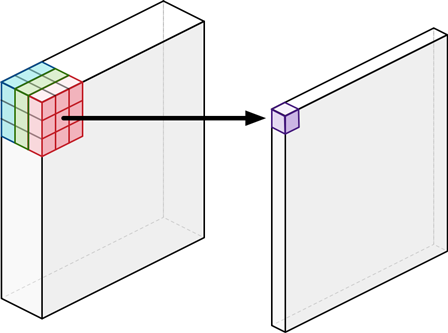
\includegraphics[scale=0.4]{conv.png}
    \caption{Принцип роботи згорткового шару $3 \times 3$ \cite{trung2019automated}}
    \label{fig:conv2d}
\end{figure}

При усіх цих перевагах згорткові мережі залишаються ефективними,
бо використовують спільні ваги для різних частин зображення.
Крім того, ми маємо змогу змінювати крок (stride) згортки, тобто параметр,
який визначає на якій відстані у пікселях будуть знаходитись ті частини
зображення до яких буде застосована згортка.
Для регуляції ж розміру вихідного зображення і ефектів, пов'язаних з
роботою операції згортки на краях зображення ми здатні використовувати
padding, тобто розширення зображення за допомогою додавання нових
пікселів з усіх боків. Значення та кількість цих пікселів залежать від
визначених архітектором мережі стратегій. Найбільш використовуваними є
варіанта заповнення нулями, або ж віддзеркалення значень з країв зображення.

Просторові ж підвибірки можливо реалізовувати або ж знову таки
за допомогою операції згортки з різними параметрами stride,
або ж за допомогою pooling. Цей метод зменшення розмірності ставить
на меті вирішення проблеми, яка пов'язана з тим, що одні й ті ж
самі ознаки можуть знаходитись у різних частинах зображення,
що призводить до різних вихідних мап ознак. Сам процес полягає у тому, що
ми певним чином для кожної мапи частини вхідної мапи ознак даємо у відповідність
одне значення, яке узагальнює ці ознаки. Найпоширенішими ж стратегіями є наступні:
\begin{enumerate}
    \item average pooling --- усереднення усіх вхідних ознак
    \item max pooling --- підрахунок найбільшого значення.
\end{enumerate}

Використовуючи вищезазначені складові блоки ми можемо
будувати архітектур нейронних мереж, які будуть ефективно застосовні
до даних у вигляді зображень та будуть відповідати усім необхідним
вимогам, які ми ставимо перед мережею.

\subsection{Архітектура UNet}

Однією з таких архітектур, що є визнаним лідером у задачі
семантичної сегментації, у тому числі, супутникових зображень є
архітектура UNet \cite{unet}.

Вона являє собою повністю згорткову (fully-convolutional) мережу, тобто
не містить ніяких інших типів шарів, окрім згортки, транспонованої згортки чи
інших методів збільшення розміру та pooling-у (і у деяких
випадках, шарів, що нормалізують). Головною ідеєю даної
архітектури, як це проілюстровано на рис. \ref{fig:unet}, є
додавання додаткових шляхів (skip connections) з шарів, які зменшують
розмір простору ознак, до шарів, які збільшують. Зменшуючи розмір простору
ознак ми з кожним кроком виділяємо все більш високорівневі
ознаки, але значна частина інформації, особливо щодо розташування
на зображенні, може бути втрачена. Застосування ж такої
архітектури дозволяє нам враховувати ознаки з різних етапів.
І крім того, у деяких випадках, подолати явище затухання градієнтів.

Особливої уваги заслуговує і той факт, що кількість каналів ознак
для кожного шару, що збільшує, залишається великою, на відміну від класичних
згорткових мереж. Це дає змогу більш ефективно враховувати контекстну
інформацію.

\begin{figure}[!ht]
    \centering
    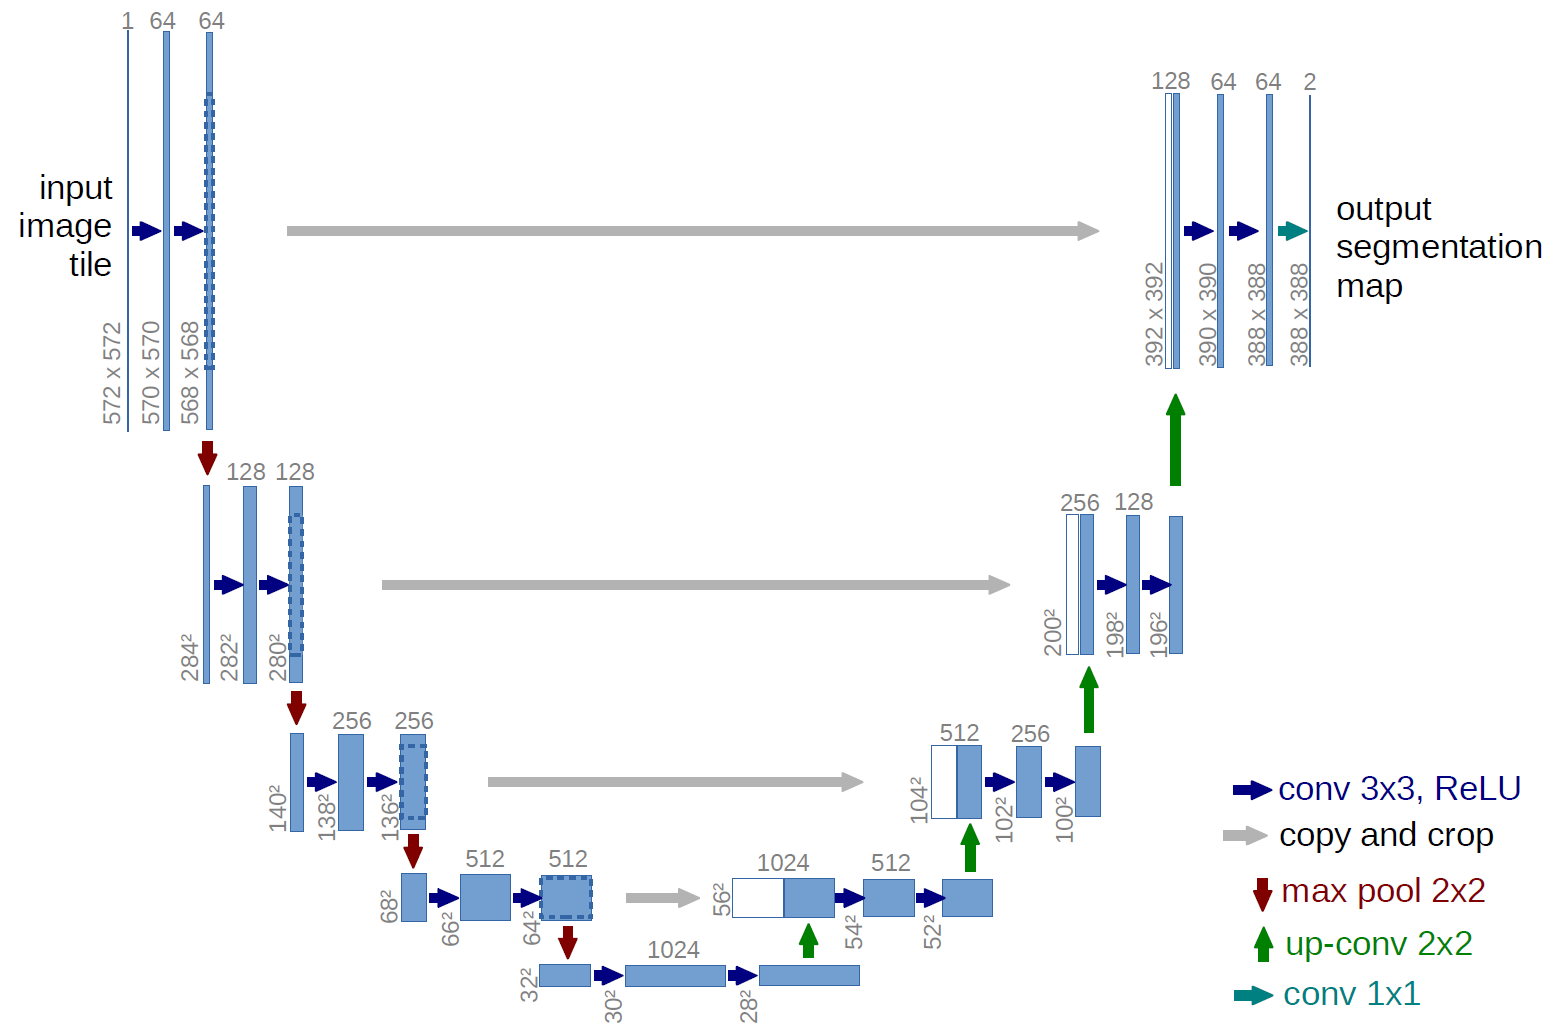
\includegraphics[width=0.8 \textwidth]{unet.png}
    \caption{Схематичне зображення \cite{unet} архітектури  UNet}
    \label{fig:unet}
\end{figure}

У класичному UNet, запропонованому у \cite{unet} кожний блок зменшення і збільшення містить 2 згорткові шари розміром $3 \times 3$, за кожним
з яких слідує ReLU активація. При чому на кожному блоці збільшення
кількість каналів подвоюється, а на кожному блоці зменшення ділиться навпіл.
Для зменшення використовується max-pooling з
кроком (stride) 2. Виходи з блоків зменшення і входи до блоків
збільшення конкатенуються, що і являє собою головну особливість архітектури.
Останній шар являє собою згортку $1 \times 1$ з кількістю ознак, яка дорівнює
кількості класів.

Проте у сучасних реальних застосуваннях, для збільшення
якості та точності сегментації дану архітектуру видозмінюють, шляхом
заміни структури блоків зменшення та збільшення. Як приклад, замість
усіх блоків зменшення можна використовувати мережу ResNet-34, при цьому
у конкатенації будуть приймати участь проміжні шари даної мережі.
Даний підхід дозволяє суттєво підвищити ефективність застосування
архітектури UNet не втративши головні її переваги.

\section{Проблеми, що виникають при застосуванні нейромережевих підходів}

Попри використання сучасних нейромережевих
архітектур, при розв'язку задач
семантичної сегментації супутникових знімків
виникають істотні проблеми, які не дозволяють
досягти максимальної якості. Ці перепони
є наслідком самої структури задачі, а саме того, що
семантична сегментація у постановці \ref{def:sem_segm_task}
є задачею навчання з учителем, тобто вимагає розміченого
набору даних, де кожному супутниковому знімку буде
відповідати відповідна ground-truth маска сегментації.

Тож першою істотною проблемою є те, що створення
навчальних вибірок, а саме: розмітка супутникових знімків,
вимагає значної кількості людських ресурсів. Причому кінцева
якість сегментації безпосередньо залежить від
розміру тренувального набору. Тобто потреба у
покращені значень метрик вимагає, серед усього іншого,
істотного збільшення навчальних прикладів,
а отже й створених людьми ground-truth масок.
Крім того, у випадку створення масок для супутникових знімків,
не завжди людина може правильно класифікувати усі об'єкти ґрунтуючись
тільки на зображенні, що може бути пов'язано з порою року,
розміром об'єкту, роздільною здатністю знімка, схожістю різних класів, тощо.

Друга істотна проблема пов'язана з дуже сильною
незбалансованістю класів, особливо у задачах класифікації
сільськогосподарських культур.
Як доказ цього, можна
навести статистику (рис. \ref{fig:pixels_per_class}) ground truth
маски по кількості пікселів по кожному з
типів полів та кількості зображень, отриманих після
поділу композиту на частини по $256 \times 256$ пікселів
на яких представлений даний клас для Київської області.
Вищезгаданий поділ обумовлений тим, що нейромережеві моделі не
можуть ефективно працювати з дуже великими зображеннями,
тож ми вимушені різати їх на частини.

\begin{figure}[ht!]
    \centering
    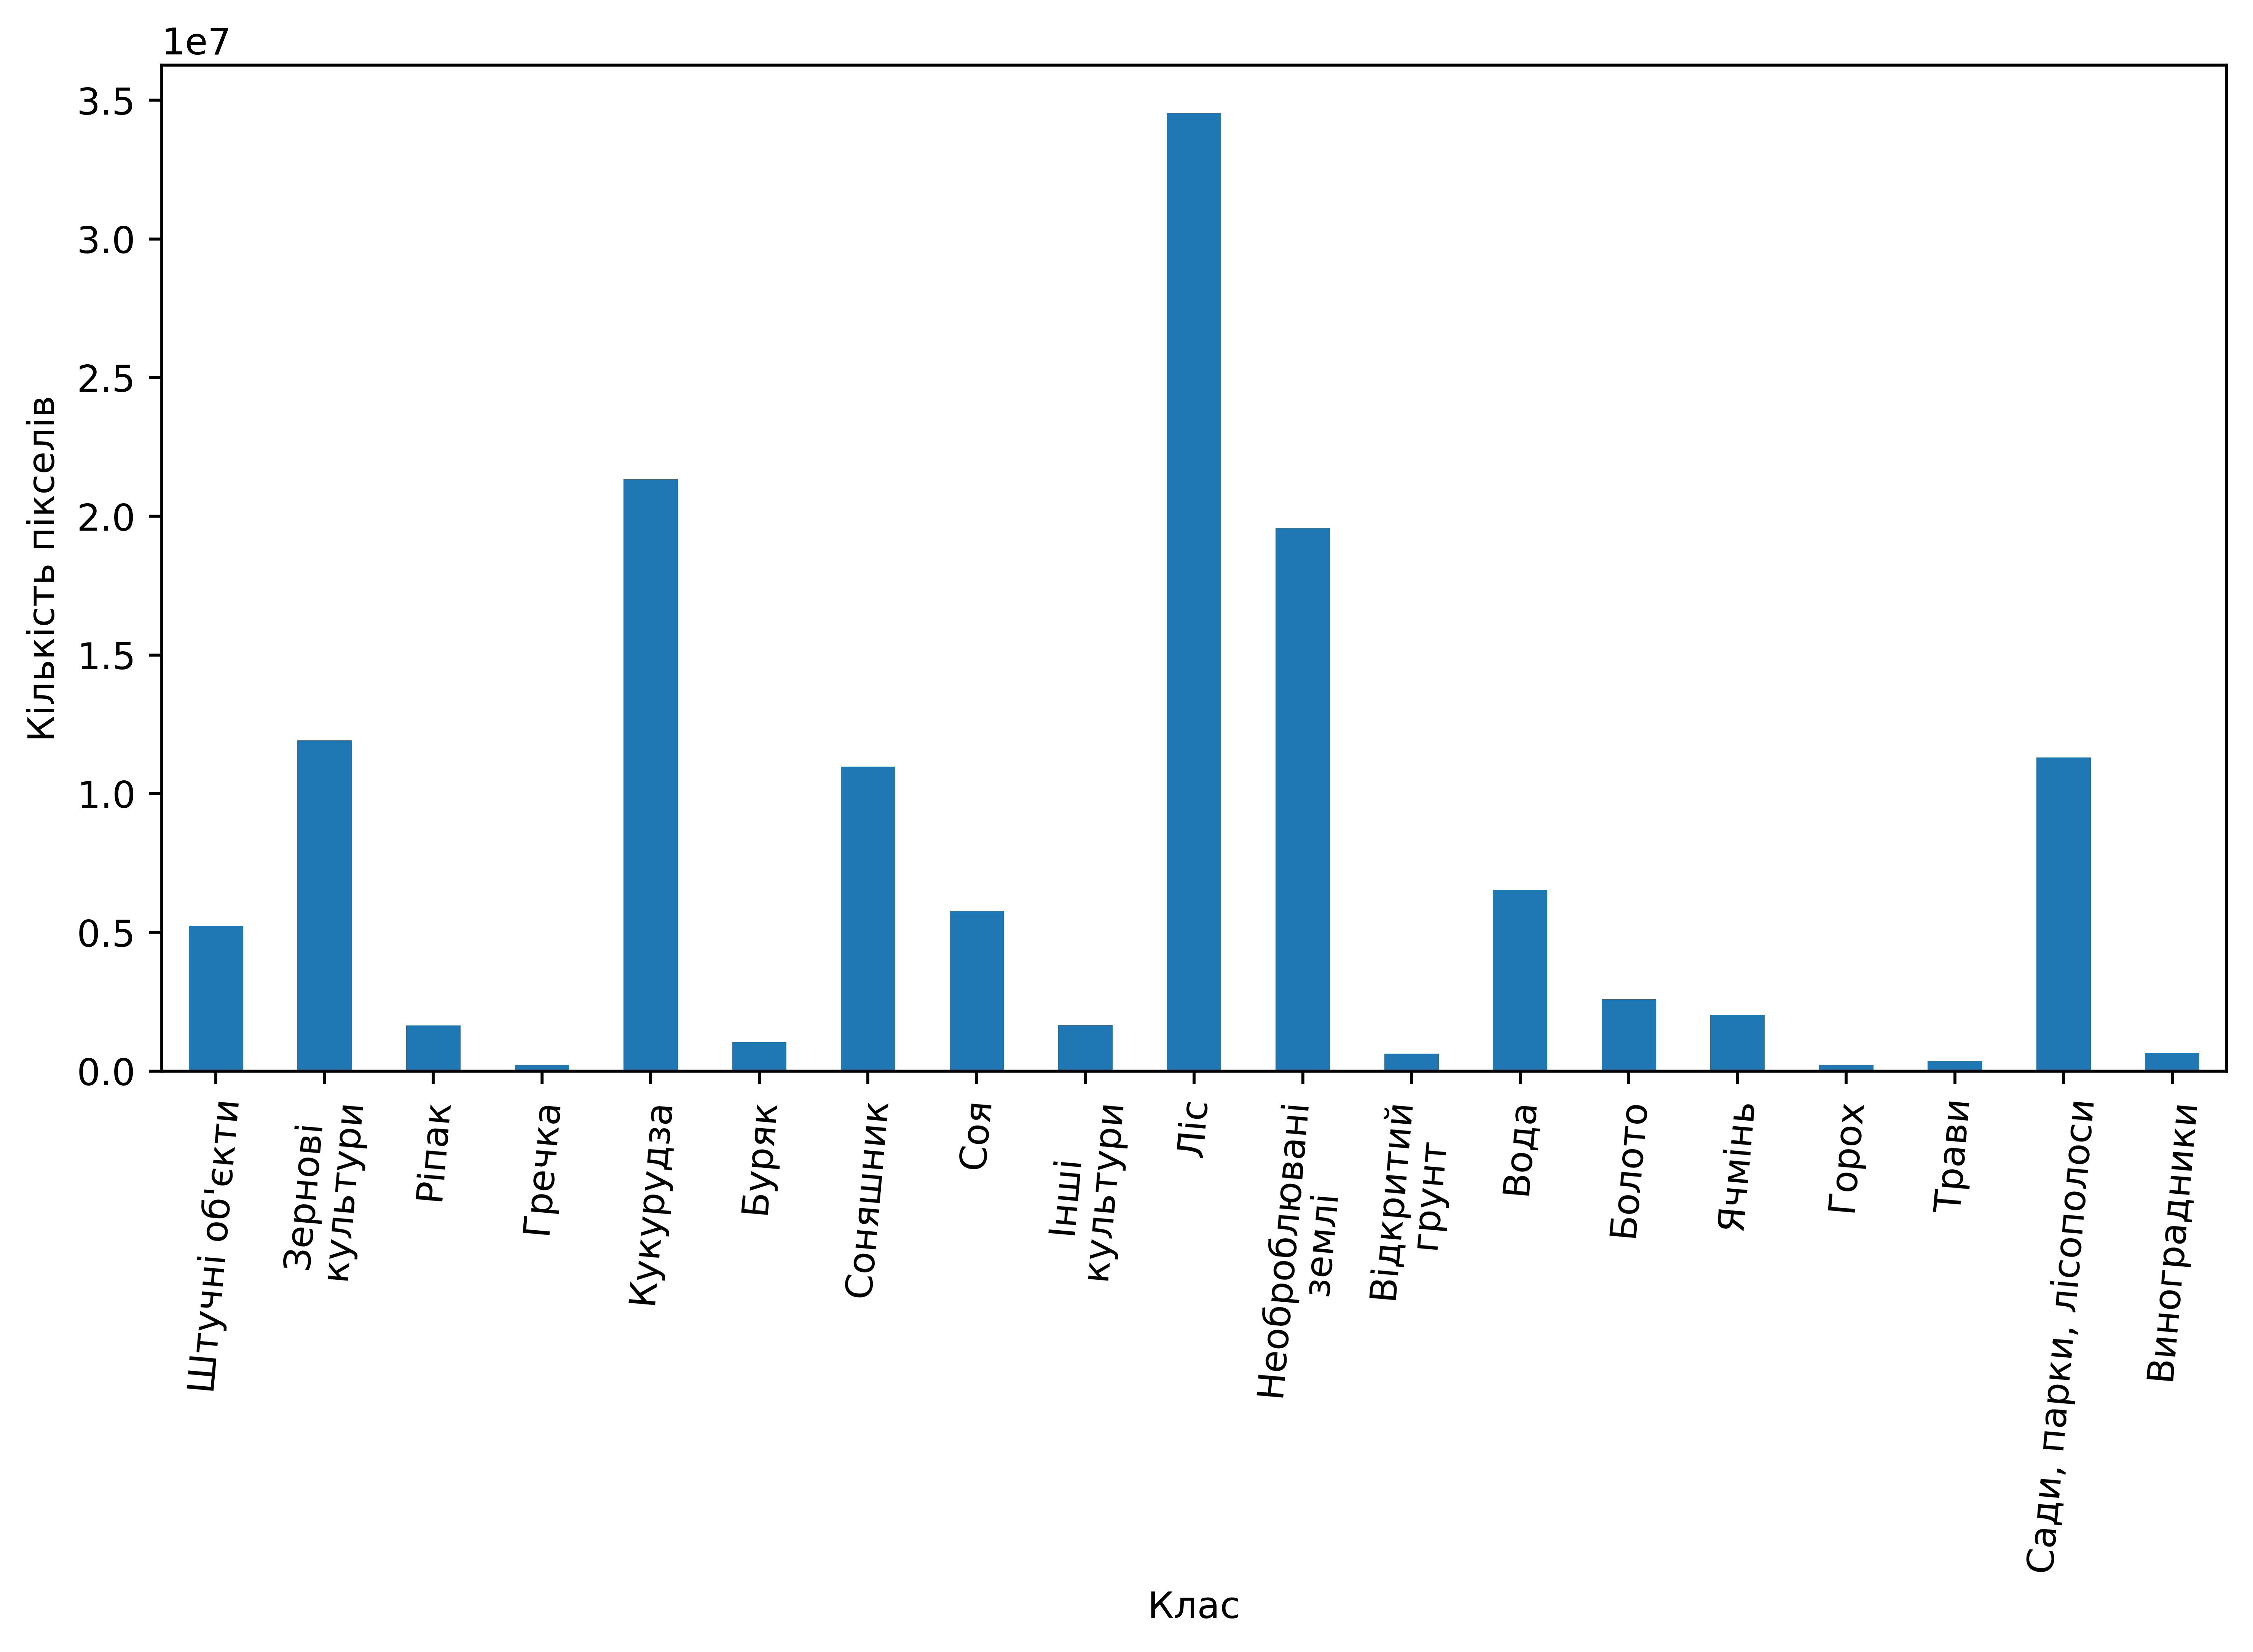
\includegraphics[scale=0.65]{dist_real.png}
    \caption{Кількість пікселів для різних класів сільськогосподарських культур
        у досліджуваному наборі даних}
    \label{fig:pixels_per_class}
\end{figure}

І попри застосування
функцій помилок, які можуть враховувати дисбаланс у
класах, досягнути бажаних значень метрик, що описують точність
моделей не вдається, що ми побачимо у подальших розділах цієї роботи.
Особливо незадовільні результати виникають саме для класів,
які мають маленьку кількість прикладів у навчальній вибірці.
А доповнити навчальну вибірку достатньою кількістю
прикладів для певних класів може бути взагалі неможливо,
через особливості сільського господарства у досліджуваному регіоні
або самої сільськогосподарської культури. Тобто знайти
ділянку земної поверхні, на якій окремий клас
буде достатньо представлений, у деяких випадках
не є можливим. Останній факт як раз
і є специфічним саме для аналізу супутникових знімків і
виділяє їх серед усіх інших сфер,
де розв'язується задача семантичної сегментації.

\chapconclude{\ref{chap:sem_segm}}
У даному розділі ми розглянули постановку задачі семантичної сегментації
супутникових знімків, яка є однією з найважливіших
задач у цій сфері, бо має багато прикладних застосувань.
Були розглянуті різні вигляди функцій помилки, а саме: крос-ентропія,
зважена крос-ентропія та Focal Loss, які можуть суттєво впливати
на якість сегментації при застосуванні сучасних методів.

Визначено й засоби оцінки та порівняння різних моделей, тобто
метрики, які застосовні до розглянутої задачі. Серед них
точність (Accuracy), User Accuracy, Producer Accuracy,
каппа Коена та міра Жаккара. Усі з перелічених метрик можливо
ефективно обрахувати використовуючи матрицю невідповідностей, і при
цьому кожна з них має зрозумілий для кінцевого користувача сенс.

Згорткові нейромережі --- це ефективний спосіб розв'язання задач,
пов'язаних з обробкою зображень, у тому числі задач семантичної
сегментації супутникових знімків. Архітектура ж UNet, яка була
розглянута у даному розділі, на даний момент є одним з найпотужніших,
визнаних науковою спільнотою підходів до цієї задачі. Вона використовує додаткові шляхи
(skip connections), щоб враховувати інформацію з мап ознак різної розмірності,
що особливо важливо при аналізі супутникових знімків.

Було виявлено, що значними проблемами при
розв'язку задачі семантичної сегментації за
допомогою сучасних нейромережевих підходів є
складність формування великих вибірок, а також,
що є специфічним для супутникових даних, сильна
незбалансованість класів, яку інколи неможливо
змінити, бо додати реальні спостереження,
з бажаним розподілом класів, не є можливим.
